\section{NVIDIA Jetson TK1 development board}
\label{sec:jetson_tk1}

Στο κεφάλαιο αυτό παρουσιάζεται η ενσωματωμένη πλατφόρμα Jetson TK1 της NVIDIA,
η οποία χρησιμοποιήθηκε για εφαρμογή των υλοποιήσεων για
\emph{Αναγνώριση και Εντοπισμό Αντικειμένων} σε συστήματα πραγματικού χρόνου,
με Νευρωνικά Δίκτυα Συνέλιξης.

Ο \emph{Tegra K1} είναι το πρώτο SOC της NVIDIA, για φορητές συσκευές, με προηγμένη αρχιτεκτονική
και χαρακτηριστικά, καθώς και χαμηλή κατανάλωση ισχύος. H μέγιστη κατανάλωση είναι στα \emph{3Watt},
τιμή που δικαιολογεί την ενσωμάτωση του σε φορητές συσκευές (tablets, smartphones), καθώς και
σε προηγμένα ενσωματωμένα συστήματα (embedded systems) για εφαρμογές πραγματικού χρόνου.

\begin{figure}[!ht]
  \centering
  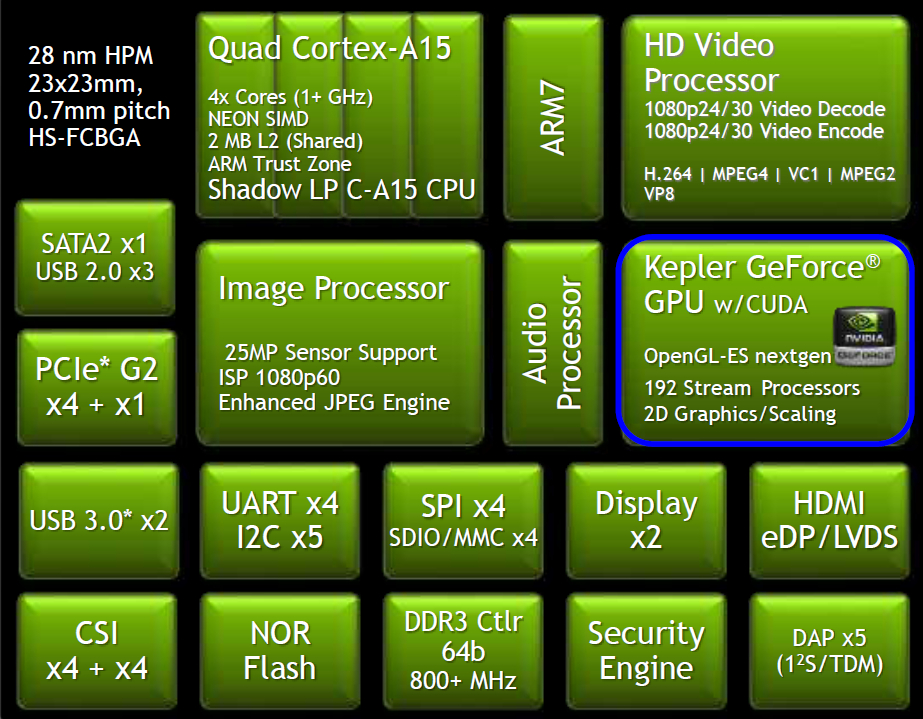
\includegraphics[width=0.7\textwidth]{./images/chapter4/nvidia_tegrak1_block2.jpg}
  \caption{Tegra K1 SOC}
  \label{fig:tegrak1soc}
\end{figure}
\noindent

Όπως φαίνεται στο \autoref{fig:tegrak1soc}, τα βασικά τεχνικά χαρακτηριστικά του Tegra K1 SOC:
\begin{itemize}
  \item{CPU: Quad-core ARM Cortex-A15 CPU, 2.3Ghz}
  \item{GPU: GK20A Kepler-based GPU with 192 CUDA cores}
  \item{RAM: DDR3L/LPDDR3, up to 8GB}
  \item{Peripherals I/O: USB, eMMC/SD-card, LVDS, HDMI, SPI, UART, I2C, SATA, PCIe}
  \item{ISP: Image processor}
\end{itemize}

Στα πλαίσια της παρούσας διπλωματικής εργασίας, επιλέχτηκε να χρησιμοποιήσουμε το
\emph{Jetson TK1} development board της NVIDIA, που φαίνετaι στο \autoref{fig:jetson_tk1}.
\begin{figure}[!ht]
  \centering
  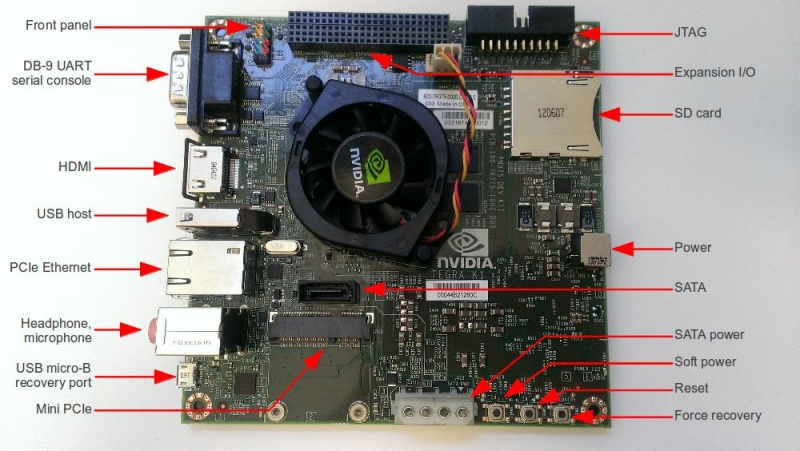
\includegraphics[width=0.9\textwidth]{./images/chapter4/jetson-tk1-labelled.jpg}
  \caption[Jetson TK1 development board]{Jetson TK1 development board}
  \label{fig:jetson_tk1}
\end{figure}
Το Jetson TK1 ενσωματώνει το Tegra K1 SOC (CPU+GPU+ISP)
και είναι πλήρες συμβατό με διάφορες διανομές λειτουργικών συστημάτων Linux (Ubuntu, Debian, Arch, Fedora, openSUSE, Gentoo).
Η πλήρης συμβατότητα και υποστήριξη λειτουργικού συστήματος Linux ήταν βασικό κριτήριο
στην επιλογή του συγκεκριμένου ενσωματωμένου συστήματος αφού επιτρέπει την
εγκατάσταση εργαλείων με τον ίδιο τρόπο όπως σε ένα σταθερό υπολογιστικό σύστημα (Desktop PC)
το οποίο τρέχει Linux OS. Πέρα από την συμβατότητα με κλασσικές διανομές Linux OS,
η NVIDIA έχει αναπτύξει δικό της λειτουργικό σύστημα, \emph{Linux4Tegra}, το οποίο
έχει σαν βάση τα Ubuntu-14.04, με κάποιες επεκτάσεις για πλήρη υποστήριξη του hardware του Jetson TK1.
Επιπλέον παράγοντας στην επιλογή της συγκεκριμένης πλατφόρμας είναι η πληθώρα των περιφερειακών διεπαφών που
διαθέτει, κάνοντας το χρήσιμο για εφαρμογή σε ρομποτικά συστήματα όπου η σύνδεση διαφόρων περιφερειακών συσκευών,
όπως για παράδειγμα αισθητήρες, κάμερες, κινητήρες, σερβο-κινητήρες, είναι απαίτηση.
Πιο κάτω δίνονται οι βασικές διεπαφές που προσφέρει η πλατφόρμα Jetson TK1:
\begin{itemize}
  \setlength\itemsep{0em}
  \item{mini-PCIe: Σύνδεση πρόσθετων συσκευών στον δίαυλο PCI-Express όπως, Wifi cards, SSD δίσκων, κτλ.}
  \item{USB 2.0 port: Για σύνδεση συσκευών ή/και αισθητήρων με διεπαφή eHCI (Extended Host Controller Interface)}
  \item{USB 3.0 port: Για σύνδεση συσκευών ή/και αισθητήρων με διεπαφή xHCI (eXtensible Host Controller Interface)}
  \item{HDMI: Δίνει την δυνατότητα σύνδεσης οθόνης}
  \item{RS232 port: Παρόλο που το RS232 είναι αρκετά παλιό πρωτόκολλο, εξακολουθεί να ενσωματώνεται σε διάφορες συσκευές που δεν απαιτούν μεγάλο όγκο μεταφοράς δεδομένων, όπως οι οδηγοί κινητήρων}
  \item{Audio IO}
  \item{Gigabit Ethernet LAN: Δικτύωση της πλατφόρμας με τον "έξω" κόσμο}
  \item{SATA: Επιτρέπει την σύνδεση σκληρού δίσκου SATA}
  \item{JTAG port: Το JTAG προσφέρει την δυνατότητα σύνδεσης συσκευής/προγράμματος εντοπισμού σφαλμάτων (debugger), για επαγγελματική αποσφαλμάτωση}
  \item{UART port}
  \item{I2C ports: Διαθέτει τρεις θύρες I2C για σύνδεση αισθητήρων/συσκευών που οδηγούνται με το συγκεκριμένο πρωτόκολλο}
  \item{GPIO: Προσφέρει δύο θύρες επέκτασης (expansion ports), με 50 και 75 ακροδέκτες αντίστοιχα. Χρήσιμο κυρίως για, επικοινωνία συσκευών με SPI, οδήγηση σερβο-κινητήρων, διακλάδωση τροφοδοσίας σε τρίτες συσκευές, κτλ.}
\end{itemize}

Όσον αφορά την υλοποίηση και ανάπτυξη Νευρωνικών Δικτύων σε ενσωματωμένα συστήματα,
η πλατφόρμα Jetson TK1 θεωρείται ιδανική αφού υποστηρίζει CUDA και cuDNN.
H cuDNN (CUDA Deep Neural Network library) είναι GPU-accelerated βιβλιοθήκη για Νευρωνικά Δίκτυα,
η οποία αναπτύχθηκε από την NVIDIA και προσφέρει υψηλού επιπέδου υλοποιήσεις για ρουτίνες όπως συνέλιξη,
κανονικοποίησης δεδομένων, pooling, επίπεδα ενεργοποίησης, κτλ.
Η βιβλιοθήκη cuDNN χρησιμοποιείται και ενσωματώνεται στα πιο δημοφιλή εργαλεία σχεδίασης και υλοποίησης μοντέλων DNN,
τα οποία και παρουσιάζονται στο \autoref{sec:dnn_sw}.

\begin{figure}[!ht]
  \centering
  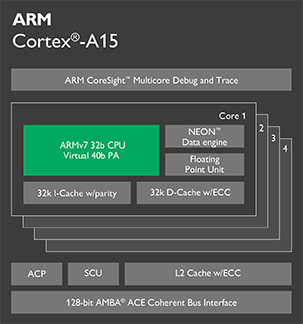
\includegraphics[width=0.6\textwidth]{./images/chapter4/cortex_A15_chip_diagram.png}
  \caption[ARM Cortex-A15 processor]{ARM Cortex-A15 processor}
  \label{fig:cortex_A15}
\end{figure}

Ένα από τα μειονεκτήματα της πλατφόρμας Jetson TK1 είναι αρχιτεκτονική των 32 bit του επεξεργαστή ARM Cortex-A15 MPCore
που έχει ενσωματωμένο (\autoref{fig:cortex_A15}). Με την εμφάνιση των επεξεργαστών ARM Cortex-A57, οι οποίοι είναι αρχιτεκτονικής 64 bit,
η υποστήριξη σε λογισμικά, τόσο από την πλευρά της NVIDIA όσο και από την ανοικτού-κώδικα (open-source) κοινότητα, μειώθηκε.
Η NVIDIA σταμάτησε να υποστηρίζει μηχανήματα αρχιτεκτονικής 32 bit, τις βιβλιοθήκες CUDA και cuDNN,
από την έκτη και δεύτερη έκδοση αντίστοιχα. Η CUDA είναι σήμερα στην έκδοση 8 και η cuDNN στην έκδοση 5,
οι οποίες φέρουν τρομερές αναβαθμίσεις στην επίδοση των αλγορίθμων βαθιάς εκμάθησης
\footnote{\href{https:/developer/nvidia/cudnn}{https:/developer/nvidia/cudnn}}.
Όπως θα δούμε στο \autoref{chapter:implementations} το γεγονός αυτό έφερε πολλά
προβλήματα καθ όλη την διάρκεια των υλοποιήσεων.
